% ============================================================
% 词对提示对大语言模型开放式生成质量的影响
% 主文档：导言区 + 标题块 + 摘要 + 章节引入
% ============================================================
\documentclass[11pt,a4paper]{article}

\usepackage[UTF8,scheme=plain]{ctex}
\usepackage{geometry}
\geometry{a4paper, top=2.5cm, bottom=2.5cm, left=2.5cm, right=2.5cm}
\usepackage{graphicx}
\usepackage{xcolor}
\usepackage{amsmath}
\usepackage{amssymb}
\usepackage{booktabs}
\usepackage{tabularx}
\usepackage{adjustbox}
\usepackage{multirow}
\usepackage{caption}
\usepackage{enumitem}
\usepackage{titlesec}
\usepackage{fancyhdr}
\usepackage{indentfirst}
\usepackage{tikz}
\usetikzlibrary{arrows.meta,positioning}
\usepackage[
    colorlinks=true,
    linkcolor=black,
    citecolor=blue!55!black,
    urlcolor=blue!55!black,
    bookmarks=true,
    bookmarksnumbered=true,
    unicode=true
]{hyperref}

% ---------- 排版细节 ----------
\widowpenalty=10000
\clubpenalty=10000
\setlength{\parskip}{0.3em}
\linespread{1.32}
\captionsetup{font=small, labelfont=bf, skip=5pt}

% ---------- 标题样式（中文期刊风格） ----------
\titleformat{\section}{\large\bfseries\heiti}{\thesection}{0.8em}{}
\titleformat{\subsection}{\normalsize\bfseries\heiti}{\thesubsection}{0.8em}{}
\titleformat{\subsubsection}{\normalsize\bfseries}{\thesubsubsection}{0.8em}{}
\titlespacing*{\section}{0pt}{1.4em plus 0.3em minus 0.1em}{0.7em}
\titlespacing*{\subsection}{0pt}{1.0em plus 0.2em minus 0.1em}{0.5em}

% ---------- 页眉页脚 ----------
\setlength{\headheight}{14pt}
\pagestyle{fancy}
\fancyhf{}
\fancyhead[L]{\small\itshape 词对提示对大语言模型开放式生成质量的影响}
\fancyhead[R]{\small\thepage}
\renewcommand{\headrulewidth}{0.4pt}

% ---------- 常用命令 ----------
\newcommand{\baseline}{\textsc{baseline}}
\newcommand{\wordpairs}{\textsc{word\_pairs}}

\begin{document}

% ============================================================
% 标题块（正文首页，封面另行生成合并）
% ============================================================
\begin{center}
{\zihao{2}\bfseries\heiti 词对提示对大语言模型开放式生成质量的影响\\[0.5em]}
{\zihao{4}\bfseries\heiti 基于 DeepSeek 双模型生成与双评委盲评的实证研究\par}
\vspace{1.2em}
{\zihao{4} 183600\textsuperscript{1}\par}
\vspace{0.3em}
{\zihao{-5} \textsuperscript{1} 独立研究者（Gitee: qwe12345678），实验数据与代码归档于\\
\url{https://gitee.com/qwe12345678/jkdsfn}（分支 \texttt{v2-deepseek}）\par}
\vspace{0.8em}
{\zihao{-5} 2026 年 10 月\par}
\end{center}
\vspace{0.6em}

\noindent\rule{\textwidth}{0.75pt}
\begin{center}
{\bfseries\heiti 摘\quad 要}
\end{center}
\noindent
针对“让大语言模型在正式作答前先输出 200 组灵感词对能否提升开放式生成质量”这一问题，本文设计并实施了一项受控实验。以 DeepSeek-V4.1-Flash 与 DeepSeek-V4-Pro 两个商用大语言模型为生成模型，在 6 个开放式生成任务上对比 \baseline{}（直接作答）与 \wordpairs{}（先输出 200 组词对再作答）两种条件，每格重复 10 次，共获得 240 条有效生成。词对条件的输出经严格协议清洗（残留引用 0 条）后，由上述两个模型作为评委对每对回答进行位置哈希平衡的 A/B 盲评，共获得 240 对有效比较。结果表明：\baseline{} 在 93.3\%（224/240）的比较中胜出，整体质量配对平均分差为 $+1.72$ 分（配对 $t$ 检验 $t=21.02$，$p<0.001$；Wilcoxon 符号秩检验 $p<0.001$）；词对提示仅在原创性维度获得小幅但统计显著的提升（平均 $+0.31$ 分，$p<0.001$），在逻辑性、具体性与可操作性三个维度均显著落后。任务分解显示原创性收益集中于概念构建型任务（如人格模型设计），而词对条件的生成 token 成本约为 \baseline{} 的 $1.60\sim2.02$ 倍，清洗后正文长度反而更短。机理分析表明，指令目标稀释、联想语境干扰与清洗信息损失是词对提示整体失效的三条主要途径。本研究为“先发散、后收敛”类提示策略的适用边界提供了可复现的实证依据，并讨论了以原创性为首要目标时该类提示的可行用法。

\vspace{0.4em}

\noindent{\bfseries\heiti 关键词：} 大语言模型；提示工程；词对提示；开放式生成；LLM 盲评；原创性评价

\noindent\rule{\textwidth}{0.75pt}
\vspace{1.0em}

\begin{center}
{\bfseries Abstract}
\end{center}
\noindent
To answer whether asking large language models (LLMs) to first output 200 inspiration word pairs before answering improves the quality of open-ended generation, we conducted a controlled experiment. Using two commercial LLMs, DeepSeek-V4.1-Flash and DeepSeek-V4-Pro, as generators, we compared the \textsc{baseline} (direct answering) condition against the \textsc{word\_pairs} condition (outputting 200 word pairs before answering) on six open-ended generation tasks, with 10 runs per cell, yielding 240 valid generations. After a strict cleaning protocol (zero residual references), the word-pair outputs were evaluated through position-balanced A/B blind comparisons by both models acting as judges, producing 240 valid paired judgments. The \textsc{baseline} won 93.3\% (224/240) of comparisons, with a mean paired overall-quality difference of $+1.72$ points (paired $t=21.02$, $p<0.001$; Wilcoxon $p<0.001$). The word-pair prime yielded only a small but significant gain in originality ($+0.31$ points, $p<0.001$) while lagging significantly in logic, concreteness, and actionability. Task-level analysis shows that originality gains concentrate in concept-construction tasks, whereas the word-pair condition costs $1.60\sim2.02\times$ more completion tokens and produces shorter post-cleaning texts. We identify goal dilution, associative-context distraction, and cleaning-induced information loss as three mechanisms underlying the overall failure of word-pair priming. The study provides reproducible empirical evidence for the applicability boundary of diverge-then-converge prompting strategies.
\vspace{0.4em}

\noindent{\bfseries Keywords:} large language models; prompt engineering; word-pair priming; open-ended generation; LLM-as-a-judge; originality evaluation

\vspace{1.2em}

% ============================================================
% 第 1 章 引言 + 第 2 章 相关工作
% ============================================================
\section{引言}

提示工程（prompt engineering）已成为无需参数更新即可调控大语言模型行为的主要手段。自思维链（chain-of-thought，CoT）提示被证明能显著提升推理任务表现以来\cite{wei2022cot,kojima2022zeroshot}，研究者提出了大量在正式作答前插入中间生成环节的策略：零样本思维链在答案前追加“请一步步思考”\cite{kojima2022zeroshot}，自一致性采样多条推理路径后投票\cite{wang2023selfconsistency}，思维树则在解题过程中显式引入分支搜索与回溯\cite{yao2023tot}。这类方法共同的隐含假设是：\textbf{模型在产出最终答案之前进行的额外生成，能够以可迁移的方式改善最终答案本身}。

然而，上述证据大多来自具有唯一正确答案的推理或问答任务。在开放式生成场景（如方案设计、创意构想、理论构建）中，“中间生成”是否同样有益，仍缺乏系统证据。一个自然但未被充分检验的猜想是：让模型在作答前先自由联想一批发散性的“灵感素材”，再基于素材作答，可以起到类似头脑风暴的作用，使答案更具原创性。本文研究的\textbf{词对提示}（word-pair priming）正是此类策略的一个典型实例——在任务指令前加入前缀：“在回答前面输出200组词，每组有两个词，从这些词获得灵感”。该策略的直觉来源是认知心理学中的发散思维与远距离联想：两个词构成的意象组合（如“潮·汐”“光·影”）可能触发模型跨越常规语义邻域的组合搜索，从而突破训练分布中的常规答案模式。

这一策略存在三重潜在风险。其一，\textbf{指令目标稀释}：200 组词对通常消耗数千 token 的生成预算，可能压缩正文的论证篇幅与细节密度；其二，\textbf{语境干扰}：已有研究表明大语言模型极易被无关上下文分散注意力\cite{shi2023distracted}，长上下文中的信息利用也存在“中间丢失”效应\cite{liu2024lost}，随机联想词对与任务的相关性参差不齐，可能将模型注意力引向低质量联想；其三，\textbf{交付形态问题}：词对列表属于过程性输出，若需从最终产物中剥离，清洗操作本身可能破坏正文的连贯性。这三条风险在推理任务中并不显著（因为推理链是答案的构成部分），但在开放式生成中被同时激活。

针对上述问题，本文基于一个公开归档的实验仓库\footnote{\raggedright 实验数据与全部原始归档位于 Gitee 仓库 \texttt{qwe12345678/jkdsfn}（分支 \texttt{v2-deepseek}，目录 \texttt{llm\_experiment\_results\_v2/}）：\par\url{https://gitee.com/qwe12345678/jkdsfn}\par}，对词对提示的有效性进行了严格的实证检验。实验以 DeepSeek-V4.1-Flash 与 DeepSeek-V4-Pro\cite{deepseekv3}两个商用模型为生成器，在 6 个开放式生成任务上比较 \baseline{} 与 \wordpairs{} 两种条件（每格 10 次重复，共 240 条生成），词对输出经带正则校验的二次清洗协议处理后，由两个模型充当评委进行位置哈希平衡的 A/B 盲评（240 对）。本研究的贡献如下：

\begin{enumerate}[leftmargin=2em, itemsep=0.15em]
  \item 提出并量化了一种“先发散素材、后正式作答”提示策略在开放式生成任务上的效果，填补了该类策略在非推理任务上的证据空白；
  \item 设计了双生成模型$\times$双评委的交叉盲评协议，并通过确定性位置平衡、清洗残留校验、数据溯源等手段控制了 LLM 评审中的主要混淆因素\cite{zheng2023judging}；
  \item 给出一致的量化结论：词对提示使整体质量平均下降 $1.72$ 分（10 分制，$p<0.001$），仅在原创性维度小幅获益（$+0.31$ 分，$p<0.001$），且代价是 $1.60\sim2.02$ 倍的生成 token 成本；
  \item 基于逐对分差、任务分解与案例文本，提出了词对提示失效的三条机理解释（目标稀释、语境干扰、清洗损失）及其适用边界。
\end{enumerate}

本文其余部分组织如下：第 2 节回顾相关工作；第 3 节给出实验设计；第 4 节报告实验结果；第 5 节进行案例分析；第 6 节讨论失效机理与实践启示；第 7 节分析有效性威胁；第 8 节总结全文。

\section{相关工作}

\subsection{思维链家族与中间生成策略}

中间生成策略的谱系始于少样本思维链提示。Wei 等人在数学、常识与符号推理任务上证明，在少样本示例中嵌入中间推理步骤可显著提升大模型表现\cite{wei2022cot}；Kojima 等人进一步发现，仅添加“让我们一步步思考”即可激活零样本推理能力，无需任何示例\cite{kojima2022zeroshot}。在解码层面，Wang 等人提出自一致性方法，对多条思维链采样后按多数答案投票，将单条路径的生成转化为集成决策\cite{wang2023selfconsistency}；Yao 等人的思维树方法则将中间推理组织为可回溯的树搜索，支持前瞻与自我评估\cite{yao2023tot}。这些方法的共同特点是：\textbf{中间生成与最终答案之间存在直接的逻辑依赖}——推理链的每一步都构成答案的推导组件。这与本文研究的词对提示形成鲜明对照：200 组灵感词对与最终正文之间不存在逻辑推导关系，仅存在启发式关联。因此，思维链家族的成功并不能外推到“自由联想素材”类提示；后者需要独立的实证检验。此外，指令微调研究指出，模型的指令遵循能力与生成目标的聚焦程度密切相关\cite{ouyang2022instructgpt}，而插入与任务无直接依赖的前置生成可能削弱这种聚焦。

\subsection{提示敏感性与无关上下文干扰}

大量证据表明大语言模型对提示的表面形式高度敏感。Sclar 等人系统量化了少-shot 提示的格式扰动（大小写、分隔符、间距）对模型表现的影响，发现性能波动可达数十个百分点，且不同模型的敏感度差异巨大\cite{sclar2024format}。Shi 等人则证明，在算术与常识推理题中加入与解题无关的句子会导致显著的性能下降，模型容易被表面相似但语义无关的上下文“带偏”\cite{shi2023distracted}。在长上下文场景下，Liu 等人发现多文档问答中位于上下文中部的信息利用率显著低于首尾，即“中间丢失”效应\cite{liu2024lost}。词对提示在结构上同时具备这三个风险因子：它向生成上下文注入数百个与任务相关性未经验证的联想项，且这些联想项在自回归生成中恰好位于正文之前（而非遥远的上下文中部），其对正文生成的持续影响缺乏先验保证。本文的实验可视为对“自生成的无关上下文”（self-generated irrelevant context）这一特殊干扰源的受控检验。

\subsection{LLM 作为评委及其偏差}

以强模型替代人工进行开放式输出评价已获得广泛验证。Zheng 等人在 MT-Bench 与 Chatbot Arena 上证明，GPT-4 级评委与人类偏好的一致率可达 80\% 以上，与人类评委之间的一致率相当\cite{zheng2023judging}；但他们同时系统识别了 LLM 评委的若干系统偏差：\textbf{位置偏差}（对 A/B 呈现顺序敏感）、\textbf{冗长偏差}（偏好更长回答）与\textbf{自我增强偏差}（偏好自家模型输出）。Shi 等人对位置偏差进行了更系统的测量，表明其在成对与列表式评审中普遍存在，交换顺序重评是有效缓解手段\cite{shi2025position}。本文的盲评协议据此进行了针对性设计：评委 prompt 明确声明“引用未展示灵感词本身不扣分”以切断对清洗残留的惩罚性归因；A/B 位置由确定性哈希平衡；采用双评委交叉评审以缓解单评委的自我增强偏差；并在结果分析中显式报告位置偏差量级（第 \ref{sec:position} 节）。此外，情感激励研究亦提示 prompt 中的额外刺激可双向影响输出质量\cite{li2023emotion}，进一步说明任何“看似无害”的提示附加物都需要实验验证而非直觉判断。

% ============================================================
% 第 3 章 实验设计
% ============================================================
\section{实验设计}\label{sec:method}

\subsection{总体架构}

实验遵循“生成—清洗—盲评”三阶段流水线（图~\ref{fig:pipeline}）。阶段 0 为生成阶段：对每个任务以两种条件各调用生成模型 10 次；阶段 1 为清洗阶段：仅对 \wordpairs{} 条件的输出剥离词对列表与正文中的词对引用；阶段 2 为盲评阶段：将同一（任务，重复）下的 \baseline{} 正文与清洗后词对正文组成一对，交由评委模型进行 A/B 盲评。两个生成模型同时充当评委，形成 $2\times2$ 的生成$\times$评审交叉设计。

\begin{figure}[htbp]
\centering
\begin{tikzpicture}[
  font=\small,
  box/.style={draw=gray!70, rounded corners=2pt, text width=2.15cm,
              minimum height=1.05cm, align=center, fill=blue!4, inner sep=2pt},
  arr/.style={-{Stealth[length=5pt]}, thick, gray!70}
]
  \node[box] (tasks) {6 个开放式\\任务};
  \node[box, right=0.72cm of tasks] (gen) {双条件生成\\$2$ 模型 $\times 2$ 条件\\$\times 10$ 次};
  \node[box, right=0.72cm of gen] (clean) {LLM 清洗\\正则校验\\二次清洗};
  \node[box, right=0.72cm of clean] (judge) {A/B 盲评\\$2$ 评委\\位置哈希平衡};
  \node[box, right=0.72cm of judge] (stats) {配对统计\\胜负 / 分差\\显著性检验};
  \draw[arr] (tasks) -- (gen);
  \draw[arr] (gen) -- (clean) node[midway, above, font=\small\bfseries, text=black] {词对输出};
  \draw[arr] (gen) to[bend right=28] node[midway, below, font=\small\bfseries, text=black] {baseline 正文} (judge);
  \draw[arr] (clean) -- (judge);
  \draw[arr] (judge) -- (stats);
\end{tikzpicture}
\caption{实验三阶段流水线。生成阶段的 \baseline{} 输出直接进入盲评，\wordpairs{} 输出需先经清洗阶段剥离词对列表与引用。}
\label{fig:pipeline}
\end{figure}

\subsection{任务集}\label{sec:tasks}

为覆盖开放式生成的不同类型，实验选取 6 个中文开放式任务（表~\ref{tab:tasks}）：T1、T3、T6 偏工程方案设计（编程语言、CLI 工具、机器学习架构），T2 偏方法论综合，T4、T5 偏概念构建（新理论、人格分类模型）。所有任务均无唯一正确答案，评价只能依赖多维度质量判断而非客观对错，这与词对提示的目标场景（提升发散产出质量）一致。任务指令保持极简（一句中文），以避免指令本身对生成施加结构约束。

\begin{table}[htbp]
\centering
\caption{实验任务与指令原文}
\label{tab:tasks}
\small
\begin{tabularx}{\textwidth}{clX}
\toprule
编号 & 主题 & 指令原文 \\
\midrule
T1 & 函数式编程语言 & 设计一个全新的函数式编程语言 \\
T2 & 提升 LLM 性能 & 怎么低成本不需要额外训练大幅提升现有 LLM 的性能 \\
T3 & CLI 工具 Idea & 给出适合独立开发者开发 CLI 工具的一个 Idea \\
T4 & 新理论 & 提出一个新的理论 \\
T5 & 人格模型 & 提出一个新的类似于九型和荣格八维的模型 \\
T6 & ML 架构 & 提出一个新的机器学习架构 \\
\bottomrule
\end{tabularx}
\end{table}

\subsection{实验条件与词对前缀}

两种条件仅相差一个前置指令。\baseline{} 条件直接输入任务指令；\wordpairs{} 条件在任务指令前附加如下前缀：

\begin{quote}
\small\itshape “在回答前面输出200组词，每组有两个词，从这些词获得灵感”
\end{quote}

前缀之后拼接原任务指令。除该前缀外，两个条件使用完全相同的模型、温度（$0.6$）、随机种子与解码参数，保证差异仅来源于前缀本身。值得强调的是，该前缀并未规定词对的领域或与任务的相关性，模型需要自行决定联想方向；这正是对“自由头脑风暴”策略的忠实模拟，也是其风险来源——没有任何机制保证 200 组联想词与任务质量相关。

\subsection{清洗协议}\label{sec:cleaning}

\wordpairs{} 输出的正文常显式引用词对（如“从上面词对中”“第 N 组的意象”），若不剥离，评委可能将其视为对不可见信息的幻觉引用而惩罚。为此，清洗阶段使用 LLM 执行严格指令：删除开头词对列表；删除或改写正文中所有依赖该词表的表述；改写后不得新增事实；只输出清洗后的正文。清洗后使用正则表达式校验残留（匹配“第 N 组 / 词组 N / 词对 N / 从上面 / 这些词中”等模式），命中者触发第二轮强化清洗，仍残留者打上 \texttt{residual} 标记。最终两个模型各 60 条清洗结果中残留均为 \textbf{0 条}，且 60/60 全部清洗成功，为盲评提供了干净的输入。清洗本身由生成模型在低温（$0.3$）下执行，与盲评温度一致。

\subsection{盲评协议}\label{sec:judge}

盲评采用成对 A/B 比较。对每个（生成模型，任务，重复）三元组，将 \baseline{} 正文与清洗后词对正文随机分配到 A/B 位置——具体由 (模型, 任务, 重复, 评委) 的确定性哈希决定，保证两端位置总体均衡且实验完全可复现。评委通过系统提示被要求以五维 1--10 整数评分并给出最终胜负（A/B/tie）：\textbf{逻辑性}（logic，逻辑与结构）、\textbf{具体性}（concreteness，细节丰富度）、\textbf{可操作性}（actionability）、\textbf{原创性}（originality）与\textbf{整体质量}（overall），并以 JSON 格式输出评分与理由。评委 prompt 中明确写入：“两篇回答都可能引用了一组未展示给您的灵感词；这种引用本身不应作为扣分理由”，以切断评委对清洗残余的惩罚性归因。

两个生成模型（V4.1-Flash、V4-Pro）各自对全部 120 对（2 生成模型 $\times$ 60 对）评审一次，形成每格 20 次、总计 240 对的评审矩阵。该交叉设计有两个作用：其一，任何一组的结论若在另一评委下复现，则可排除单评委偏好；其二，生成模型自评其输出构成的格子（如 V4-Pro 评审 V4-Pro 生成）可与交叉格子对比，检验自我增强偏差的影响。

\subsection{实现细节与数据完整性}

实验通过 DeepSeek 官方 API（\texttt{api.deepseek.com/v1}，OpenAI 兼容接口）于 2026-10-22 执行，运行标识 \texttt{v2-deepseek-20261022T235120Z}，全局随机种子 20261022。每条记录附完整溯源字段（\texttt{schema\_version}、\texttt{run\_id}、时间戳、模型、\texttt{prompt\_version}、种子），生成与清洗温度为 $0.6$ 与 $0.3$。数据完整性如下：生成阶段 $2\times120=240$ 条记录全部有效（0 条错误）；清洗阶段两模型各 60 条，全部成功且 0 残留；盲评阶段 240 对全部解析成功。全部原始数据、逐条 markdown 与汇总脚本均归档于公开仓库\footnote{生成正文、清洗结果与盲评理由的逐条归档位于仓库 \texttt{llm\_experiment\_results\_v2/} 目录，共 720 个 markdown 文件与 6 个 JSONL 数据文件。}，支持独立复核。

\subsection{评价指标与统计方法}\label{sec:metrics}

报告四类指标。（1）\textbf{胜负频次}：各（生成模型 $\times$ 评委）格子的 \baseline{} 胜、\wordpairs{} 胜、平局计数。（2）\textbf{五维平均分}：按格子报告两条件在五个维度上的均值。（3）\textbf{配对分差}：对每次比较 $i$，定义第 $d$ 维配对分差
\begin{equation}\label{eq:diff}
\Delta_i^{(d)} = S^{\,(d)}_{\text{base},i} - S^{\,(d)}_{\text{wp},i},
\end{equation}
其中 $S^{\,(d)}_{\text{base},i}$、$S^{\,(d)}_{\text{wp},i}$ 分别为该次评审中 \baseline{} 与 \wordpairs{} 文本在第 $d$ 维的得分。注意分差按“\baseline{} 减 \wordpairs{}”定向，正值表示 \baseline{} 更优。对合并的 240 个配对，报告 $\Delta^{(d)}$ 的均值、标准差、中位数与正/零/负计数，并用配对 $t$ 检验与 Wilcoxon 符号秩检验（剔除零差）检验 $\Delta^{(d)}=0$ 原假设；两个检验分别响应分差的近似正态性与秩结构，结论一致时推断更稳健。（4）\textbf{成本指标}：生成阶段的完成 token 数与耗时，以及清洗阶段的长度压缩比（清洗后字符数 / 原始字符数）。位置偏差通过 A 位与 B 位平均分之差 $\bar S_A - \bar S_B$ 及条件化分差（A 为 \baseline{} 时、A 为 \wordpairs{} 时的 A$-$B 分差）度量。

% ============================================================
% 第 4 章 实验结果
% ============================================================
\section{实验结果}\label{sec:results}

\subsection{总体胜负}\label{sec:wins}

表~\ref{tab:wins} 汇总了四个（生成模型 $\times$ 评委）格子的盲评胜负。在全部 240 对有效比较中，\baseline{} 胜出 224 对（93.3\%），\wordpairs{} 仅胜 15 对（6.3\%），平局 1 对。四个格子的结论高度一致：最“接近”的格子（V4.1-Flash 生成、V4-Pro 评审）中 \wordpairs{} 也仅获 8/60 胜；差距最大的格子（V4-Pro 生成）中 \wordpairs{} 仅 1/60 胜。若剔除唯一平局并做二项符号检验，239 次非平局比较中 \baseline{} 获胜 224 次，显著性远超常规阈值（$p<10^{-40}$）。这与先验概率 0.5 的“无差异”假设形成强烈对比：\textbf{在所考察的开放式生成场景中，词对提示几乎总是降低最终产物的竞争力}。

\begin{table}[htbp]
\centering
\caption{盲评胜负汇总（每格 60 对；行 = 生成模型，列属性 = 评委）}
\label{tab:wins}
\small
\begin{tabular*}{\textwidth}{@{\extracolsep{\fill}} l l r r r r}
\toprule
生成模型 & 评委模型 & \baseline{} 胜 & \wordpairs{} 胜 & 平局 & \wordpairs{} 胜率 \\
\midrule
V4.1-Flash & V4.1-Flash & 54 & 5 & 1 & 8.3\% \\
V4.1-Flash & V4-Pro    & 52 & 8 & 0 & 13.3\% \\
V4-Pro    & V4.1-Flash & 59 & 1 & 0 & 1.7\% \\
V4-Pro    & V4-Pro    & 59 & 1 & 0 & 1.7\% \\
\midrule
\multicolumn{2}{l}{\textbf{合并}} & \textbf{224} & \textbf{15} & \textbf{1} & \textbf{6.3\%} \\
\bottomrule
\end{tabular*}
\end{table}

值得注意的两个跨格子规律。第一，\textbf{生成模型越强，词对提示伤害越大}：V4-Pro 生成时 \wordpairs{} 胜率从 8.3\%--13.3\% 跌至 1.7\%。一个直观解释是：强模型的 \baseline{} 输出本身已具备较高的结构完整性与细节密度，留给前置联想环节的改进空间更小，而词对带来的目标稀释代价不变甚至相对更大。第二，\textbf{交叉评审与自评格子的结论几乎相同}（V4-Pro 生成时，两个评委均给出 59/1/0），未观察到明显的自我增强偏差影响胜负方向的现象。

\subsection{五维平均分}\label{sec:scores}

表~\ref{tab:dims} 报告各格子两条件在五个维度上的平均分，图~\ref{fig:radar} 以雷达图呈现双评委均值。四个格子呈现一致的形态：\baseline{} 在逻辑性、具体性、可操作性与整体质量四个维度全面占优，\wordpairs{} 仅在原创性维度部分反超。以合并配对视角（第 \ref{sec:diff} 节），唯一方向相反的维度正是原创性。

\begin{table}[htbp]
\centering
\caption{五维平均分（10 分制；按生成模型 $\times$ 评委分组，$n=60$/格）}
\label{tab:dims}
\small
\begin{tabular*}{\textwidth}{@{\extracolsep{\fill}} l l l r r r r r}
\toprule
生成模型 & 评委 & 条件 & 逻辑性 & 具体性 & 可操作性 & 原创性 & 整体 \\
\midrule
\multirow{4}{*}{V4.1-Flash} & \multirow{2}{*}{V4.1-Flash} & \baseline{} & 8.97 & 8.87 & 8.78 & 7.53 & 8.88 \\
 &  & \wordpairs{} & 7.95 & 7.40 & 6.88 & \textbf{8.05} & 7.62 \\
\cline{2-8}
 & \multirow{2}{*}{V4-Pro} & \baseline{} & 9.00 & 8.92 & 8.85 & 7.68 & 8.87 \\
 &  & \wordpairs{} & 7.92 & 7.62 & 7.20 & \textbf{8.33} & 7.82 \\
\midrule
\multirow{4}{*}{V4-Pro} & \multirow{2}{*}{V4.1-Flash} & \baseline{} & 8.93 & 8.82 & 8.47 & 7.42 & 8.78 \\
 &  & \wordpairs{} & 6.95 & 6.05 & 5.58 & 7.20 & 6.40 \\
\cline{2-8}
 & \multirow{2}{*}{V4-Pro} & \baseline{} & 9.02 & 9.02 & 8.57 & 7.52 & 8.80 \\
 &  & \wordpairs{} & 6.93 & 6.25 & 5.73 & \textbf{7.82} & 6.62 \\
\bottomrule
\end{tabular*}
\end{table}

\begin{figure}[htbp]
\centering
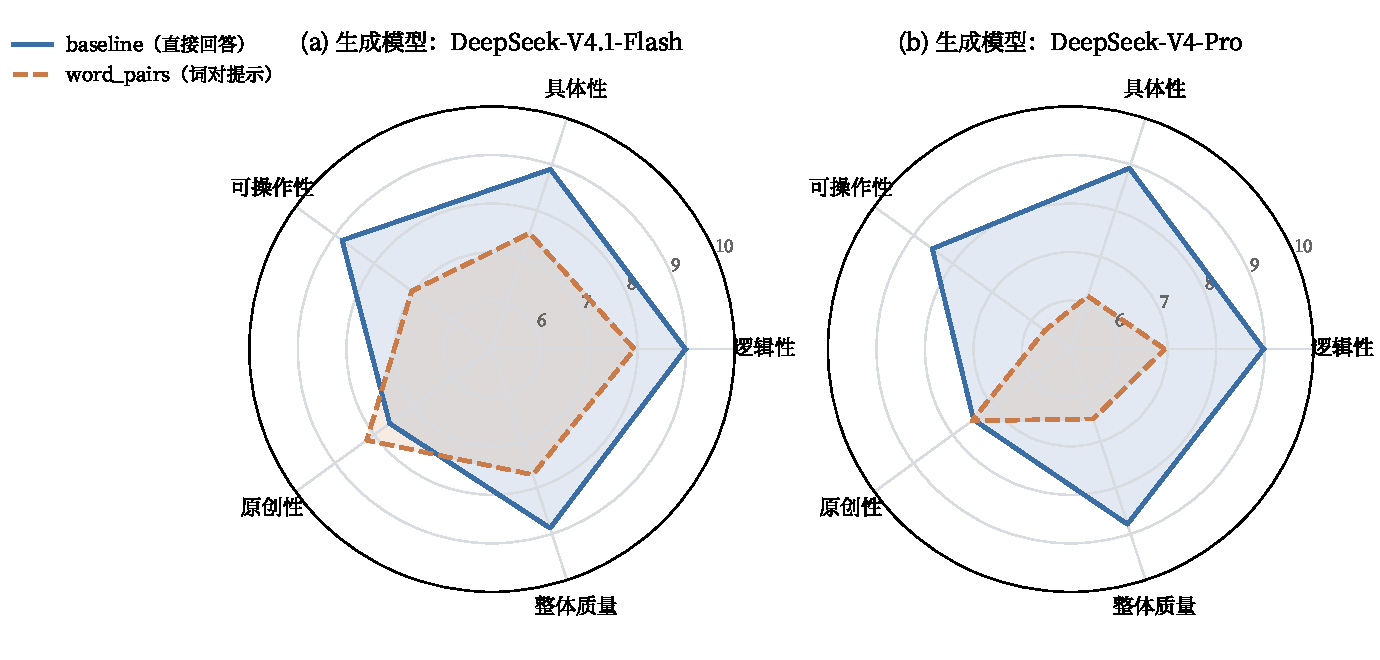
\includegraphics[width=\textwidth]{figs/fig_radar.pdf}
\caption{五维平均分雷达图（双评委均值，10 分制）。虚线（\wordpairs{}）仅在原创性轴超出实线（\baseline{}）。(a) V4.1-Flash 生成；(b) V4-Pro 生成。}
\label{fig:radar}
\end{figure}

维度间的受损幅度存在清晰梯度：受损最重的是\textbf{可操作性}（V4-Pro 生成时低至 5.58--5.73，较 \baseline{} 下降 $2.8\sim2.9$ 分），其次是\textbf{具体性}（下降 $2.8$ 分左右）与\textbf{逻辑性}（下降 $1.0\sim2.1$ 分）。原创性则是唯一出现正增益的维度，且增益幅度（$+0.5\sim+0.7$）明显小于其他维度的损失幅度。这一“原创性小幅增益、其余维度大幅受损”的模式在两个生成模型、两个评委下完全复现，构成了词对提示效果画像的核心。

\subsection{配对分差与显著性检验}\label{sec:diff}

逐对配对分差（式~\eqref{eq:diff}）比格子均值更能刻画分布形态。表~\ref{tab:tests} 报告 240 对合并样本五个维度的分差统计量与两项检验结果；图~\ref{fig:dist} 展示整体质量与原创性两个维度的分差直方图。

\begin{table}[htbp]
\centering
\caption{合并配对分差 $\Delta^{(d)}$ 的统计检验（$n=240$；正值表示 \baseline{} 更优；Wilcoxon 检验剔除零差后进行）}
\label{tab:tests}
\small
\begin{tabular*}{\textwidth}{@{\extracolsep{\fill}} l r r r r r r r}
\toprule
维度 & 均值 & 标准差 & 中位数 & 正/零/负 & $t$ & $p$（配对 $t$） & $p$（Wilcoxon） \\
\midrule
逻辑性   & $+1.54$ & 1.23 & 1 & 204/29/7  & 19.42  & $<10^{-50}$ & $<10^{-34}$ \\
具体性   & $+2.08$ & 1.52 & 2 & 214/14/12 & 21.10  & $<10^{-55}$ & $<10^{-35}$ \\
可操作性 & $+2.32$ & 1.57 & 2 & 220/8/12  & 22.88  & $<10^{-61}$ & $<10^{-37}$ \\
原创性   & $-0.31$ & 1.25 & 0 & 71/62/107 & $-3.88$ & $1.3\times10^{-4}$ & $8.8\times10^{-5}$ \\
整体质量 & $+1.72$ & 1.27 & 2 & 224/1/15  & 21.02  & $<10^{-55}$ & $<10^{-36}$ \\
\bottomrule
\end{tabular*}
\end{table}

\begin{figure}[htbp]
\centering
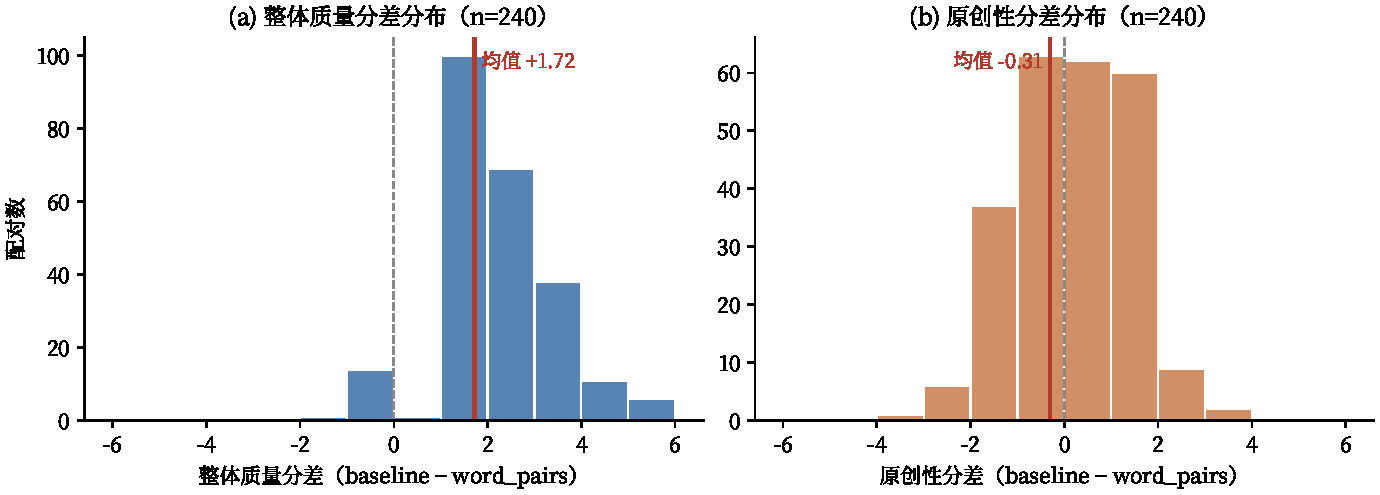
\includegraphics[width=\textwidth]{figs/fig_dist.pdf}
\caption{配对分差分布（$n=240$）。(a) 整体质量分差集中于正值区（均值 $+1.72$）；(b) 原创性分差分布近似对称且略偏负（均值 $-0.31$，即 \wordpairs{} 略优）。}
\label{fig:dist}
\end{figure}

结果有三点值得强调。第一，\textbf{整体质量的差异在统计上极端显著}：配对 $t=21.02$（$p\approx3\times10^{-56}$），Wilcoxon $p\approx4\times10^{-37}$；两项检验基于不同假设得出一致结论，且分差分布（图~\ref{fig:dist}a）并非由少数极端离群对驱动，而是整体右移、中位数为 $+2$。第二，\textbf{原创性维度的反向效应虽小但稳定显著}：均值 $-0.31$（即 \wordpairs{} 平均高 $0.31$ 分），107 对为负、71 对为正、62 对为零（$p\approx8.8\times10^{-5}$）。效应方向与幅度均与胜负分析一致。第三，各维度的零差比例差异揭示了评价行为特征：原创性维度出现 62 次零差（25.8\%），远高于其他维度（3.3\%--12.1\%），说明评委在原创性上的分辨粒度较粗、常给出同分；而整体质量维度仅 1 次零差，因为评委被强制给出胜负结论。

\subsection{任务异质性}\label{sec:tasks-hetero}

图~\ref{fig:task} 按任务分解 \wordpairs{} 的胜场（每柱满分 20，虚线为随机水平 10）。两个模型呈现相同的不均匀格局：\textbf{六个任务中五个任务的词对胜场接近于零}（V4-Pro 生成时 T1--T4、T6 全部为 0/20），唯一例外是 \textbf{T5 人格模型}——V4.1-Flash 生成时获得 7/20 胜，虽仍未过半，却远高于其余五个任务的 1--2/20（Fisher 精确检验 $p=1.2\times10^{-3}$）；V4-Pro 生成时也仅在 T5 获得胜场（2/20）。合并双模型后，T5 贡献了全部 15 场胜局中的 9 场（$p=1.0\times10^{-4}$），是词对策略唯一具有实质竞争力的任务。

\begin{figure}[htbp]
\centering
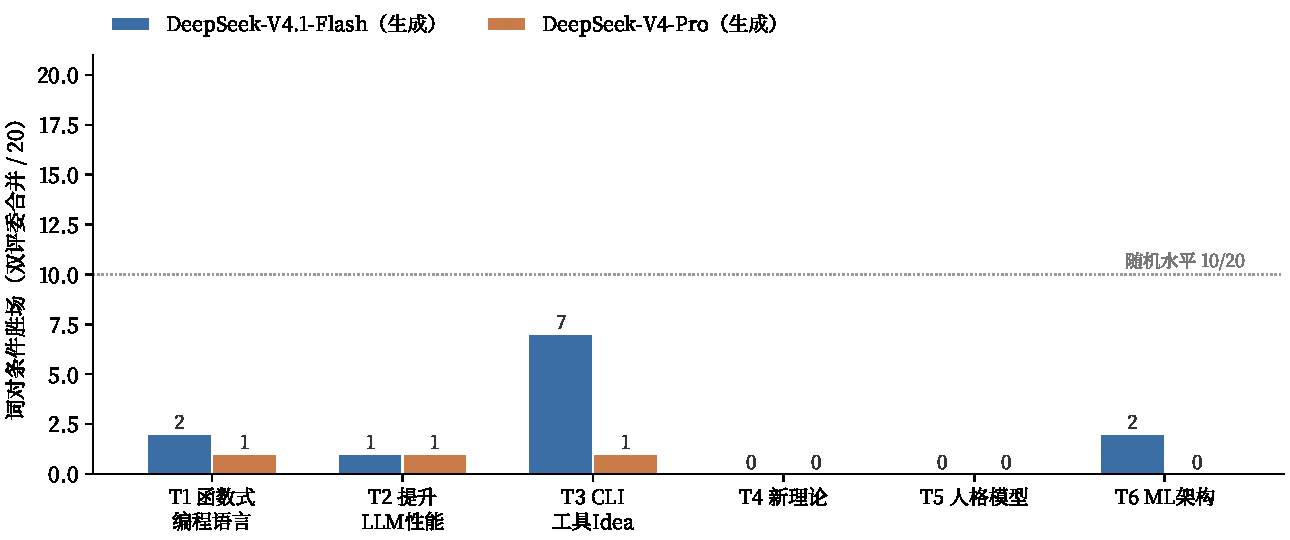
\includegraphics[width=0.92\textwidth]{figs/fig_task.pdf}
\caption{按任务分解的 \wordpairs{} 胜场（双评委合并，每柱满分 20）。虚线为 50\% 随机水平。T5（人格模型）的胜场远高于其余任务，贡献全部 15 胜中的 9 胜。}
\label{fig:task}
\end{figure}

T5 的特殊性可以从任务性质解释。人格模型设计（“提出一个新的类似于九型和荣格八维的模型”）是一个\textbf{概念构建型}任务：产出的核心价值在于提出一套自洽、有辨识度的分类学隐喻（轴、相、枢、介质等），而非工程可落地性；且该领域存在九型人格、MBTI、荣格八维等大量先例，模型的 \baseline{} 输出容易落入既有框架（评委理由中多次出现“更像成熟模型的组合”），原创性天花板受限。词对联想恰好在该任务上补足了短板：随机意象（潮汐、编织、光谱）为分类学提供了新鲜的命名与结构隐喻。这与第 \ref{sec:scores} 节“原创性是唯一受益维度”的发现互相印证：\textbf{词对提示的价值集中在“新颖性本身即核心价值”的任务上}。相反，T1/T3/T6 等工程方案类任务对可行性、技术细节的要求刚性更强，联想词无法弥补细节密度的损失。

\subsection{生成与清洗成本}\label{sec:cost}

词对提示不仅损失质量，还显著增加成本（表~\ref{tab:cost}、图~\ref{fig:cost}）。生成 token 方面，V4.1-Flash 的 \wordpairs{} 条件平均消耗 8252 个完成 token，是 \baseline{}（4089）的 \textbf{2.02 倍}；V4-Pro 为 1.60 倍（9796 对 6123）。耗时方面分别为 1.57 倍（37.5 s 对 23.9 s）与 1.36 倍（119.9 s 对 88.1 s）。清洗阶段进一步引入成本：清洗调用本身消耗 token，且词对输出中有 57\%--64\% 的字符（词对列表与相关引用）被剥离——V4.1-Flash 的压缩比为 0.43，V4-Pro 为 0.36。

\begin{table}[htbp]
\centering
\caption{生成与清洗成本（均值 $\pm$ 标准差；长度为字符数；压缩比 = 清洗后/原始长度）}
\label{tab:cost}
\small
\begin{tabular*}{\textwidth}{@{\extracolsep{\fill}} l l r r r r}
\toprule
生成模型 & 条件 & 完成token & 耗时/s & 输出长度 & 清洗后长度（压缩比） \\
\midrule
\multirow{2}{*}{V4.1-Flash} & \baseline{}   & $4090\pm2520$ & $23.9\pm12.5$ & $2774\pm1302$ & --- \\
 & \wordpairs{} & $8252\pm2767$ & $37.5\pm12.5$ & $4319\pm1100$ & $1960\pm$（0.43） \\
\midrule
\multirow{2}{*}{V4-Pro} & \baseline{}     & $6123\pm3396$ & $88.1\pm42.3$ & $3576\pm1652$ & --- \\
 & \wordpairs{} & $9796\pm2956$ & $119.9\pm48.6$ & $4090\pm1148$ & $1588\pm$（0.36） \\
\bottomrule
\end{tabular*}
\end{table}

\begin{figure}[htbp]
\centering
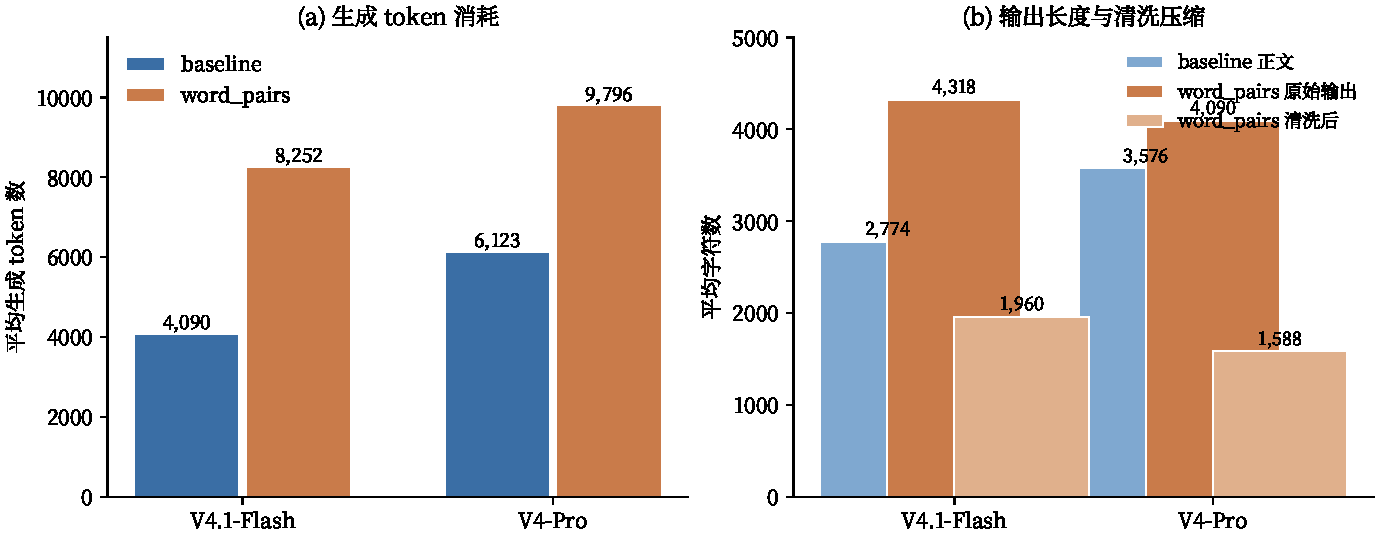
\includegraphics[width=\textwidth]{figs/fig_cost.pdf}
\caption{生成与清洗成本对比。(a) 平均完成 token 数：\wordpairs{} 条件为 \baseline{} 的 1.60--2.02 倍；(b) 输出长度与清洗压缩：清洗后的词对正文（浅色）反而短于 \baseline{} 正文。}
\label{fig:cost}
\end{figure}

最值得关注的发现是\textbf{长度反转}：词对条件的原始输出更长（字符数 4090--4319 对 2774--3576），但剥离词对与引用后，其正文长度（1588--1960）反而\textbf{显著短于} \baseline{} 正文——V4-Pro 生成时仅为 \baseline{} 的 44\%。换言之，词对提示把生成长度预算的过半数消耗在了被丢弃的过程性内容上，正文的信息密度与展开程度双降。这也部分解释了具体性与可操作性的大幅受损：在上下文长度与生成预算双重受限下，词对列表直接挤占了正文的技术细节空间。

\subsection{位置偏差分析}\label{sec:position}

表~\ref{tab:position} 报告 A/B 位置偏差。四个格子中三个出现 A 位均值高于 B 位（差值 $+0.16\sim+0.58$ 分），一个格子相反（$-0.18$ 分），平均 A 位优势约 $+0.27$ 分，量级远小于条件主效应（$+1.72$ 分）。条件化分差显示了两面性：当 \baseline{} 位于 A 位时 A$-$B 分差（$+1.42\sim+2.77$）大于 \wordpairs{} 位于 A 位时的分差绝对值（$-0.59\sim-2.14$），提示 A 位优势与条件效应存在部分叠加，可能使观测到的 \baseline{} 胜率略有高估。但即便在最保守的估计下（假设位置效应完全单向叠加），其幅度（$<0.6$ 分）也不足以解释 $93.3\%$ 的胜率与 $+1.72$ 的整体分差；且位置已由确定性哈希平衡，两组条件在 A 位的比例接近对半，位置偏差对两条件是对称的。综上，\textbf{位置偏差不改变本研究的方向性结论}。

\begin{table}[htbp]
\centering
\caption{评委位置偏差（A/B 位平均分与条件化分差）}
\label{tab:position}
\small
\begin{tabular*}{\textwidth}{@{\extracolsep{\fill}} l l r r r r}
\toprule
生成模型 & 评委 & $\bar S_A$ & $\bar S_B$ & \shortstack{A$-$B 分差\\（A 位为 \baseline{}）} & \shortstack{A$-$B 分差\\（A 位为 \wordpairs{}）} \\
\midrule
V4.1-Flash & V4.1-Flash & 8.33 & 8.17 & $+1.65$ & $-0.97$ \\
V4.1-Flash & V4-Pro    & 8.60 & 8.08 & $+1.42$ & $-0.59$ \\
V4-Pro     & V4.1-Flash & 7.50 & 7.68 & $+2.75$ & $-2.14$ \\
V4-Pro     & V4-Pro    & 8.00 & 7.42 & $+2.77$ & $-1.60$ \\
\bottomrule
\end{tabular*}
\end{table}

\subsection{与前版实验的对比}

本实验（v2）是同一研究问题第二版协议的执行结果，前版（v1）使用单一生成模型（Kimi-K3，经 NVIDIA NIM 端点）且清洗协议较弱。表~\ref{tab:v1} 汇总两版结果：v1 中 \baseline{} 胜 49/60，但 17/60 的清洗样本残留词对引用，其“\baseline{} 大幅占优”的结论存在混淆——残留引用可能被评委当作幻觉。v2 将清洗残留降为 0，并引入双生成模型、双评委与位置哈希平衡，\baseline{} 胜率反而\textbf{上升}至 93.3\%。这说明 v1 的结论并非清洗伪影所致：在彻底消除残留引用、且评委被明确告知“引用本身不扣分”的条件下，词对条件的整体劣势依然存在甚至更加清晰。两版实验在原创性维度上也一致（v1：7.15 对 8.25；v2：词对略优），进一步支持了该方向性发现。

\begin{table}[htbp]
\centering
\caption{与前版实验（v1）的协议与结果对比}
\label{tab:v1}
\small
\begin{tabular*}{\textwidth}{@{\extracolsep{\fill}} l l l}
\toprule
项目 & v1 & v2（本文） \\
\midrule
生成模型 & Kimi-K3（单模型） & V4.1-Flash + V4-Pro \\
评委 & 同一生成模型（单一） & 两个模型交叉（各评一次） \\
有效比较数 & 60 & 240 \\
清洗残留 & 17/60 & \textbf{0/120} \\
位置平衡 & 随机交换 & 确定性哈希平衡 \\
\baseline{} : \wordpairs{} : 平 & 49 : 10 : 1 & 224 : 15 : 1 \\
\bottomrule
\end{tabular*}
\end{table}

% ============================================================
% 第 5 章 案例分析 + 第 6 章 讨论 + 第 7 章 有效性威胁 + 第 8 章 结论
% ============================================================
\section{案例分析}\label{sec:case}

为理解量化结果背后的文本机制，本节选取一组典型的同源对比进行细读：V4.1-Flash 生成、T1（函数式编程语言）任务、第 1 次重复。该对由 V4-Pro 评审，\baseline{} 正文以 9/7（整体/原创）胜出。两篇输出的对比如图~\ref{fig:case}所示（节选）。

\begin{figure}[htbp]
\centering
\begin{minipage}[t]{0.485\textwidth}
\centering
\fcolorbox{gray!60}{gray!6}{\begin{minipage}{0.94\textwidth}
\small
\textbf{\baseline{}：Aster（星芒）}\par\vspace{0.3em}
``下面给出一份\textbf{可落地的}函数式编程语言设计草案。语言名为 Aster（星芒）：默认纯函数、强类型、显式效应、结构化并发、布局语法。\par
……\par
``Aster 是一门：默认纯函数式的语言；严格求值、默认不可变；使用代数数据类型 + 模式匹配；使用类型与效应行显式描述副作用；内建结构化并发；\textbf{小核心、大标准库，适合脚本、服务端和 WASM}。''\par
……\par
随后依次给出语法、类型系统（效应行）、并发模型、\textbf{实现路线图}与迁移策略等章节。
\end{minipage}}
\end{minipage}\hfill
\begin{minipage}[t]{0.485\textwidth}
\centering
\fcolorbox{gray!60}{orange!8}{\begin{minipage}{0.94\textwidth}
\small
\textbf{\wordpairs{}（清洗后）：潮织（Tideweave）}\par\vspace{0.3em}
``\textbf{潮织}是一种纯函数式、静态类型、以\textbf{效应光谱、潮汐并发、织纹模块、线性契约}为核心的实验性函数式编程语言。\par
……\par
``副作用被建模为效应光谱，用处理器进行折射与消解；结构化并发模型 tide 像潮汐一样汇聚、取消、回流结果；模块、类型和模式匹配采用织纹组合方式……''\par
……\par
正文围绕上述意象组织，术语新颖，但工程细节（实现路线、迁移策略）明显更简略。
\end{minipage}}
\end{minipage}
\caption{T1 任务第 1 次重复的两篇输出节选（V4.1-Flash 生成，V4-Pro 评审）。评审给分：Aster 整体 9 / 原创 7；潮织整体 7 / 原创 9。}
\label{fig:case}
\end{figure}

该案例浓缩了全局模式。\baseline{} 产物（Aster）从一开始就围绕“可落地”组织：非目标清单、类型与效应系统、实现路线图等章节一应俱全，评委理由为“结构更清晰、细节更具体，提供了明确的语法、类型系统、效应处理、并发模型和实现路线图，可落地的完整度更高”。\wordpairs{} 产物（潮织）则表现出鲜明的\textbf{意象驱动}特征：词对中的“潮·汐”“线·结”“织·梭”“光·谱”被系统性地转译为语言机制命名（tide 并发、织纹模块、效应光谱），评委承认其“隐喻和术语原创性更强”（原创性 9 对 7），但同时指出“在若干设计细节和可操作性上不如（\baseline{}）清晰”（可操作性 6 对 9）。这组九分制细节说明词对提示的作用通道确实存在——它把模型的搜索空间拉向了训练分布中更少出现的意象组合——但该收益以牺牲工程严谨性为代价，在多维度加权后净效应为负。

对 240 条评委理由的定性归纳显示，\baseline{} 的获胜理由高频出现“结构（更完整/清晰）”“细节（更具体/充分）”“可落地/可操作”“MVP（边界明确）”“路线图”等词；\wordpairs{} 的 15 次胜出理由则几乎全部集中于“（概念）更完整自洽”“原创整合度”“结构更丰富的分类学”等表述，且多数出现在 T5（人格模型）任务上。例如一条 T5 的评委理由写道：“A（\wordpairs{}）的模型结构更完整：八枢以四轴组织，九相由三动机核$\times$三调节流生成，并补充顺流、逆流、跨核代偿、影子枢…… 逻辑闭环与可操作性更强”。这与定量发现（T5 是唯一高于随机水平的任务）互为印证。

\section{讨论}\label{sec:discussion}

\subsection{词对提示为何整体失效：三条机制}

\textbf{机制一：指令目标稀释与预算挤占。}词对前缀实际上向模型同时下达了两个目标（先产出 200 组词、再完成任务），而两者共享同一生成预算与同一注意力资源。实验观测到三重挤占证据：(1) \wordpairs{} 条件完成 token 为 \baseline{} 的 $1.60\sim2.02$ 倍，说明词对环节本身消耗了大量生成预算；(2) 清洗后正文长度反而只有 \baseline{} 正文的 44\%--71\%，说明正文的绝对展开量下降；(3) 受损最重的维度恰是对“展开程度”最敏感的可操作性与具体性。对经过指令微调的模型而言，“先做 A 再做 B”的复合指令天然诱导对 A 的过度投入\cite{ouyang2022instructgpt}——词对是逐条枚举型内容，枚举的边际成本低而模型有完成清单的强倾向，正文于是成为预算的剩余部分。

\textbf{机制二：联想语境的自干扰。}词对列表一旦生成，就成为正文的直接上文。Shi 等人证明模型极易被无关上下文分散\cite{shi2023distracted}，而本研究中的“无关”并非人工注入而是模型自生成——这带来一个微妙的自增强回路：模型倾向于让自己的正文“呼应”刚写下的词对（潮织案例中的意象转译即为证据），哪怕这种呼应并不服务于任务质量。当联想词与任务高度相关时该回路可能有益；但 200 组无约束联想的期望相关性很低，多数词对成为正文生成时需要绕开的噪声。同时，正文需要在概念上锚定这些意象（评委观察到词对正文偏好“命名驱动”而非“问题驱动”的结构），进一步偏离了开放式任务的评价准则。

\textbf{机制三：清洗的信息损失。}与思维链不同，词对环节被设计为可剥离的“脚手架”。但正文的组织方式在生成时已与词对深度耦合（“如第 N 组词所示”“从上述意象中获得灵感”是正文的骨架性连接词），清洗协议在删除这些指代时必须改写句子，即使零残留达标，句法上的缝合痕迹与论证链的中断仍然存在——这从清洗后正文更短（压缩比 0.36--0.43）与逻辑性维度的显著受损（$+1.5$ 分分差）中可见一斑。v1 实验中 17/60 的显性残留则说明，当清洗不彻底时评委还会额外惩罚“引用不可见信息”，这是该策略在工程实现上的又一脆弱点。

\subsection{词对提示何时可能有价值}

本研究的结果并非全盘否定发散式提示，而是刻画了其适用边界。\textbf{第一，原创性维度存在真实且显著的正效应}（$+0.31$ 分，$p<0.001$），说明“自由联想素材”确实能把模型推离常规解空间。\textbf{第二，收益集中于概念构建型任务}：T5（人格模型）上 \wordpairs{} 获得 7/20 的胜场（V4.1-Flash 生成），贡献了全部 15 场胜局中的 9 场，是唯一具有实质竞争力的任务格；该类任务的产出核心是“新颖而自洽的分类学隐喻”，恰是随机意象能直接供给的原料。\textbf{第三，强模型从中获益更少}：V4-Pro 生成时各任务胜场均趋近于零。据此可以给出实践建议：若任务以新颖概念为核心价值且对工程细节不敏感（起名、世界观设定、创意写作中的意象拓展），可考虑小规模使用词对式预热，但应将词对数量降至远小于 200（减少预算挤占）、显式约束词对与任务的相关性（降低自干扰）、或干脆把“发散”与“收敛”拆分为两轮独立调用（让收敛阶段从干净上下文开始，规避清洗损失）。若任务要求可落地方案，则应避免该策略。

\subsection{对提示工程与 LLM 评审方法学的启示}

本研究的证据强化了一个更一般的判断：\textbf{“作答前的额外生成”并非免费}。思维链的成功依赖于中间内容与答案之间的逻辑依赖；一旦前置内容与任务只存在启发式关联（词对、情绪刺激\cite{li2023emotion}、自由联想），其收益就必须与目标稀释、自干扰与后处理损失相权衡，且该权衡很可能为负。对方法学而言，本研究亦示范了一个低成本但严格的评估闭环：交叉双评委消除单一评委偏好、确定性哈希平衡消除位置偏差、正则校验的二次清洗消除交付伪影、全量溯源数据支持独立复核——该协议可直接复用于其他提示策略的评估。位置偏差的测量结果（A 位平均 $+0.27$ 分，方向不完全一致）也再次印证了 Zheng 等人关于 LLM 评委偏差可控但必须显式测量的观点\cite{zheng2023judging,shi2025position}。

\section{有效性威胁}\label{sec:threats}

\textbf{LLM 评委的效度。}本研究完全依赖 LLM 盲评，未包含人工评估。尽管交叉双评委设计、与人类偏好一致性的既有证据\cite{zheng2023judging}以及 v1/v2 两版协议的复现性缓解了单评委风险，评委与人类专家在“原创性”这类主观维度上的判断仍可能存在系统差异。特别是，评委可能对工程完整性存在与任务无关的固有偏好，从而压低意象驱动文本的整体分。\textbf{冗长偏差的反向作用。}LLM 评委通常偏好更长回答\cite{zheng2023judging}，本研究中 \wordpairs{} 清洗后正文反而更短，故冗长偏差只会\emph{低估}词对条件的劣势——即真实差距可能更大，方向性结论不受影响。\textbf{模型家族单一。}两个生成模型均来自 DeepSeek 家族（V4.1-Flash 与 V4-Pro）\cite{deepseekv3}，同源模型的指令遵循与生成风格可能共享相同的失效模式；结论向其他家族模型的外推需要进一步验证（v1 使用 Kimi-K3 得到方向一致的结果，提供了初步的跨家族证据）。\textbf{语言与任务单一。}全部任务与输出均为中文，任务均为一次性开放式生成；其他语言、多轮对话或更长篇幅场景下的表现未考察。\textbf{清洗伪影。}尽管清洗残留为 0，无法完全排除“清洗改写本身而非词对策略”造成部分质量损失的可能；将该损失从策略总效应中剥离需要“对 \baseline{} 输出施加同强度改写”的对照组，这是未来工作的方向之一。\textbf{单一前缀形式。}实验仅测试了一种词对前缀（200 组、两个词、无领域约束）；词对数量、关联度约束与呈现形式的变化可能改变结论，本文结论严格限定于该具体形式。

\section{结论}\label{sec:conclusion}

本文对“作答前先输出 200 组灵感词对”这一发散式提示策略进行了双模型、双评委的受控盲评实验。在 240 条生成与 240 对盲评中，\baseline{} 以 93.3\% 的胜率、$+1.72$ 分的整体质量分差（$p<0.001$）全面占优；词对提示仅在原创性维度获得 $+0.31$ 分的显著增益，集中于概念构建型任务，代价是 $1.60\sim2.02$ 倍的生成成本与清洗后正文的信息密度下降。机理分析将其失效归因于指令目标稀释、联想语境自干扰与清洗信息损失三条通路。

本研究的核心信息是：\textbf{“先发散、后收敛”的直觉不能不加检验地移植到提示设计中}。前置发散素材只有在“新颖性本身即任务核心价值、且发散内容与任务相关性受控”的条件下才可能净收益为正。未来工作包括：(1) 引入人工评估与多模型家族交叉验证；(2) 系统变化词对数量、领域约束与生成-收敛两阶段分离方式，绘制该策略的完整设计空间；(3) 将本协议扩展到其他“过程性前置生成”策略（如情绪刺激、角色扮演预热）的统一评估，为提示工程提供更一般的设计准则。


% ============================================================
% 参考文献
% ============================================================
\begin{thebibliography}{99}
\zihao{-5}
\setlength{\itemsep}{0.2em}

\bibitem{wei2022cot}
Wei J, Wang X, Schuurmans D, et al.
Chain-of-thought prompting elicits reasoning in large language models[C]//
Advances in Neural Information Processing Systems (NeurIPS 2022). 2022: 24824--24837.
arXiv:2201.11903.

\bibitem{kojima2022zeroshot}
Kojima T, Gu S S, Reid M, et al.
Large language models are zero-shot reasoners[C]//
Advances in Neural Information Processing Systems (NeurIPS 2022). 2022: 22199--22213.
arXiv:2205.11916.

\bibitem{wang2023selfconsistency}
Wang X, Wei J, Schuurmans D, et al.
Self-consistency improves chain of thought reasoning in language models[C]//
International Conference on Learning Representations (ICLR 2023). 2023.
arXiv:2203.11171.

\bibitem{yao2023tot}
Yao S, Yu D, Zhao J, et al.
Tree of thoughts: Deliberate problem solving with large language models[C]//
Advances in Neural Information Processing Systems (NeurIPS 2023). 2023.
arXiv:2305.10601.

\bibitem{sclar2024format}
Sclar M, Choi Y, Tsvetkov Y, et al.
Quantifying language models' sensitivity to spurious features in prompt design or: How I learned to start worrying about prompt formatting[C]//
International Conference on Learning Representations (ICLR 2024). 2024.
arXiv:2310.11324.

\bibitem{shi2023distracted}
Shi F, Chen X, Misra K, et al.
Large language models can be easily distracted by irrelevant context[C]//
International Conference on Machine Learning (ICML 2023). 2023: 31220--31236.
arXiv:2302.00093.

\bibitem{liu2024lost}
Liu N F, Lin K, Hewitt J, et al.
Lost in the middle: How language models use long contexts[J]//
Transactions of the Association for Computational Linguistics, 2024, 12: 157--173.
arXiv:2307.03172.

\bibitem{zheng2023judging}
Zheng L, Chiang W L, Sheng Y, et al.
Judging LLM-as-a-judge with MT-Bench and Chatbot Arena[C]//
Advances in Neural Information Processing Systems (NeurIPS 2023), Datasets and Benchmarks Track. 2023.
arXiv:2306.05685.

\bibitem{shi2025position}
Shi L, Zhao H, Zhang Y, et al.
A systematic study of position bias in LLM-as-a-judge[C]//
Proceedings of IJCNLP-AACL 2025. 2025: 312--335.

\bibitem{ouyang2022instructgpt}
Ouyang L, Wu J, Jiang X, et al.
Training language models to follow instructions with human feedback[C]//
Advances in Neural Information Processing Systems (NeurIPS 2022). 2022: 27730--27744.
arXiv:2203.02155.

\bibitem{li2023emotion}
Li Y, Li Y, Yuan Y, et al.
Large language models understand and can be improved by emotion stimuli[J].
arXiv preprint arXiv:2307.11760, 2023.

\bibitem{deepseekv3}
DeepSeek-AI.
DeepSeek-V3 technical report[J]. arXiv preprint arXiv:2412.19437, 2024.

\bibitem{deepseekr1}
DeepSeek-AI.
DeepSeek-R1: Incentivizing reasoning capability in LLMs via reinforcement learning[J].
arXiv preprint arXiv:2501.12948, 2025.

\end{thebibliography}

% ---------- PDF 元数据 ----------
\hypersetup{
    pdftitle={词对提示对大语言模型开放式生成质量的影响},
    pdfauthor={183600},
    pdfsubject={大语言模型提示工程实证研究},
    pdfkeywords={大语言模型, 提示工程, 词对提示, 开放式生成, LLM盲评, 原创性}
}

\end{document}
